\chapter{Example 1}\label{example-1}
	
	\subsection{Problem description}\label{example-1-problem}
	
	A technology firm is planning its strategy for the next year and must choose exactly one of three possible options.
	One option is to innovate (Strategy A) by launching a new, cutting-edge product. Another option is to improve the current product line
	(Strategy B) by upgrading and refining what the firm already sells. The third option is to license an external technology (Strategy C)
	instead of developing new technology in-house.
	
	The firm knows that future market demand is uncertain and can be in one of three states high demand, moderate demand or low demand.
	Based on market research, management estimates that the probability of high demand is \(0.30\), the probability of moderate demand is \(0.40\)
	and the probability of low demand is \(0.30\). These probabilities are treated as the best available information before any decision is made.
	
	For each combination of strategy and demand, the firm has an estimate of the profit measured in thousands of dollars.
	If demand is high, the expected profits are \(150\) for Innovate (A), \(110\) for Improve (B) and \(70\) for License (C).
	If demand is moderate, the expected profits are \(80\) for Innovate (A), \(90\) for Improve (B) and \(70\) for License (C).
	If demand is low, the expected profits are \(-20\) for Innovate (A), \(40\) for Improve (B) and \(60\) for License (C).
	The firm wants to analyse this decision using several decision-making rules, including expected value, maximax, maximin
	and the maximum opportunity minimax regret criterion, and then determine which strategy provides the most coherent choice
	given its view of risk and the available probability information.
	
	\subsection{Solution}
	
	\subsubsection{(C2) Interpreting the parts of the decision problem}\label{example-1-c2}
	
	We identify the key elements and summarise them in a table.
	
	\begin{center}
		\begin{tabular}{@{}p{0.28\linewidth}p{0.62\linewidth}@{}}
			\toprule
			Element & Description \\
			\midrule
			Decision alternatives & Innovate (A), Improve (B), License (C) \\
			States of nature & High demand, Moderate demand, Low demand \\
			Fortuitous events & The actual market demand that will occur, which is unknown when deciding \\
			Consequences & Profit in thousands of dollars for each strategy--demand combination \\
			Probabilities & High demand \(0.30\), Moderate demand \(0.40\), Low demand \(0.30\) \\
			\bottomrule
		\end{tabular}
	\end{center}
	
	\subsubsection{(C3) Building the payoff table from the description}\label{example-1-c3}
	
	From the problem description, we construct the payoff table (profits in thousands of dollars).
	
	\begin{center}
		\begin{tabular}{@{}p{0.26\linewidth}p{0.14\linewidth}p{0.16\linewidth}p{0.16\linewidth}p{0.16\linewidth}@{}}
			\toprule
			State of Nature & Probability & Innovate (A) & Improve (B) & License (C) \\
			\midrule
			High demand     & \(0.30\) & 150  & 110 & 70 \\
			Moderate demand & \(0.40\) & 80   & 90  & 70 \\
			Low demand      & \(0.30\) & -20  & 40  & 60 \\
			\bottomrule
		\end{tabular}
	\end{center}
	
	\subsubsection{(C4) Maximax rule decision making without probabilities}\label{example-1-c4}
	
	We ignore probabilities and focus only on the best possible payoff for each strategy.
	
	Best payoff for each strategy
	\[
	\begin{aligned}
		\max_i \text{Payoff}(A, S_i) &= 150k\\
		\max_i \text{Payoff}(B, S_i) &= 110k\\
		\max_i \text{Payoff}(C, S_i) &= 70k
	\end{aligned}
	\]
	The largest of these is \(150k\), so the Maximax rule recommends \emph{Innovate (A)}.
	
	\subsubsection{(C5) Maximin rule decision making without probabilities}\label{example-1-c5}
	
	Now we ignore probabilities and focus on the worst-case payoff of each strategy.
	
	Worst payoff for each strategy
	\[
	\begin{aligned}
		\min_i \text{Payoff}(A, S_i) &= -20k\\
		\min_i \text{Payoff}(B, S_i) &= 40k\\
		\min_i \text{Payoff}(C, S_i) &= 60k
	\end{aligned}
	\]
	We then pick the strategy with the highest of these worst outcomes
	\[
	\max\{-20, 40, 60\} = 60k
	\]
	The Maximin rule recommends \emph{License (C)}.
	
	\subsubsection{(C6) Maximum opportunity criterion minimax regret}\label{example-1-c6}
	
	We construct the regret (opportunity loss) table. For each state of nature, we compare each payoff
	with the best payoff in that state.
	
	Best payoff in each state
	\[
	\begin{aligned}
		\text{High demand} &:\ \max\{150, 110, 70\} = 150k\\
		\text{Moderate demand} &:\ \max\{80, 90, 70\} = 90k\\
		\text{Low demand} &:\ \max\{-20, 40, 60\} = 60k
	\end{aligned}
	\]
	
	Regrets are computed as best payoff minus actual payoff.
	
	\begin{center}
		\begin{tabular}{@{}p{0.28\linewidth}p{0.20\linewidth}p{0.20\linewidth}p{0.20\linewidth}@{}}
			\toprule
			State of Nature & Innovate (A) & Improve (B) & License (C) \\
			\midrule
			High demand     & \(150-150=0\) & \(150-110=40\) & \(150-70=80\) \\
			Moderate demand & \(90-80=10\)  & \(90-90=0\)    & \(90-70=20\) \\
			Low demand      & \(60-(-20)=80\) & \(60-40=20\) & \(60-60=0\) \\
			\bottomrule
		\end{tabular}
	\end{center}
	
	Maximum regret for each strategy
	\[
	\begin{aligned}
		\max_i \text{Regret}(A, S_i) &= \max\{0, 10, 80\} = 80\\
		\max_i \text{Regret}(B, S_i) &= \max\{40, 0, 20\} = 40\\
		\max_i \text{Regret}(C, S_i) &= \max\{80, 20, 0\} = 80
	\end{aligned}
	\]
	The minimax regret rule chooses the strategy with the smallest maximum regret, so the
	maximum opportunity criterion recommends \emph{Improve (B)}.
	
	\subsubsection{(C7) Using probabilities and expected value Bayes decision rule}\label{example-1-c7}
	
	We apply the Expected Monetary Value (EMV) rule. For each strategy, we multiply each payoff by the probability
	of its state and add the results.
	
	For Innovate (A)
	\[
	\begin{aligned}
		EMV_A &= 0.30(150) + 0.40(80) + 0.30(-20) \\
		&= 0.30\cdot150 + 0.40\cdot80 + 0.30\cdot(-20) \\
		&= 45 + 32 - 6 = 71k
	\end{aligned}
	\]
	
	For Improve (B)
	\[
	\begin{aligned}
		EMV_B &= 0.30(110) + 0.40(90) + 0.30(40) \\
		&= 0.30\cdot110 + 0.40\cdot90 + 0.30\cdot40 \\
		&= 33 + 36 + 12 = 81k
	\end{aligned}
	\]
	
	For License (C)
	\[
	\begin{aligned}
		EMV_C &= 0.30(70) + 0.40(70) + 0.30(60) \\
		&= 0.30\cdot70 + 0.40\cdot70 + 0.30\cdot60 \\
		&= 21 + 28 + 18 = 67k
	\end{aligned}
	\]
	
	Under the Bayes EMV rule, the best strategy is the one with the highest EMV, so EMV recommends
	\emph{Improve (B)} with \(81k\).
	
	\subsubsection{(C9) Tree diagram of the decision-making problem}\label{example-1-c9}
	
	We represent the same situation as a decision tree.
	
	\begin{center}
		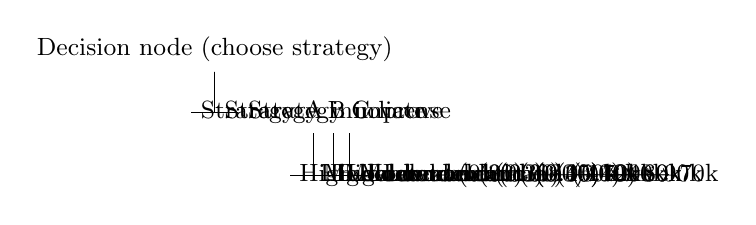
\begin{tikzpicture}[
			grow=down,
			level distance=8mm,
			sibling distance=3mm,
			edge from parent/.style={draw},
			edge from parent path={(\tikzparentnode.south) |- (\tikzchildnode.west)},
			every node/.style={anchor=west,font=\small}
		]
			\node {Decision node (choose strategy)}
				child { node {Strategy A innovate}
					child { node {High demand (0.30) $\to$ 150k} }
					child { node {Moderate demand (0.40) $\to$ 80k} }
					child { node {Low demand (0.30) $\to$ -20k} }
				}
				child { node {Strategy B improve}
					child { node {High demand (0.30) $\to$ 110k} }
					child { node {Moderate demand (0.40) $\to$ 90k} }
					child { node {Low demand (0.30) $\to$ 40k} }
				}
				child { node {Strategy C license}
					child { node {High demand (0.30) $\to$ 70k} }
					child { node {Moderate demand (0.40) $\to$ 70k} }
					child { node {Low demand (0.30) $\to$ 60k} }
				};
		\end{tikzpicture}
	\end{center}
	
	This diagram helps visualise all possible paths decisions followed by demand realisations and the associated payoffs.
	
	\subsubsection{(C8) Comparing Bayes, Maximin, Maximax and minimax regret}\label{example-1-c8}
	
	Summary of recommendations from the different rules
	\begin{itemize}
		\item Bayes EMV expected value with probabilities, no experimentation recommends \emph{Improve (B)}.
		\item Maximum opportunity minimax regret recommends \emph{Improve (B)}.
		\item Maximax very optimistic, ignores probabilities recommends \emph{Innovate (A)}.
		\item Maximin very cautious, ignores probabilities recommends \emph{License (C)}.
	\end{itemize}
	
	Bayes and minimax regret use the full payoff structure (and, in the case of Bayes, the probabilities) to favor a more balanced option,
	whereas Maximax and Maximin focus only on the most extreme possible outcomes.
	
	\subsubsection{(C10) Evaluating all possibilities in the decision problem}\label{example-1-c10}
	
	Considering all the strategies and rules together, the firm can reflect on the consequences of each possible choice.
	Innovate (A) offers the highest possible payoff but also the lowest worst-case payoff and a high maximum regret.
	License (C) protects strongly against the worst case but sacrifices expected profit and is not favoured by EMV or regret.
	Improve (B) is the only strategy that is simultaneously supported by expected value and by the minimax regret rule.
	This evaluation shows how different attitudes toward risk and regret lead to different recommended actions,
	and highlights Improve (B) as a compromise between risk and return.
	
	\subsubsection{(C1) Formulating the final decision and summarising all criteria}\label{example-1-c1}
	
	Based on each of the worked decision criteria, the recommended decision would be as follows.
	
	If the firm decides according to the Maximax rule (C4) and is willing to act with a very optimistic, risk-seeking attitude,
	it should choose \emph{Innovate (A)} because this strategy has the highest possible payoff among all options.
	
	If the firm decides according to the Maximin rule (C5) and adopts a very conservative, worst-case oriented perspective,
	it should choose \emph{License (C)} since this strategy has the strongest worst-case payoff.
	
	If the firm decides according to the maximum opportunity minimax regret rule (C6) and wants to minimise the largest possible regret,
	it should choose \emph{Improve (B)} because this strategy has the smallest maximum regret.
	
	If the firm decides according to the Bayes EMV rule (C7) using the estimated probabilities and focusing on long-run average profit,
	it should again choose \emph{Improve (B)} because it has the highest expected monetary value.
	
	The decision tree (C9) does not change the recommendation but confirms, in a visual and systematic way,
	the same payoffs and probabilities used in these rules.
	
	Finally, the comparison in (C8) and the global evaluation in (C10) show that each rule corresponds to a particular attitude
	toward risk and uncertainty.
	
	Taking all criteria together, a coherent summary conclusion is that the strategy \emph{Improve (B)}
	provides the most balanced decision for this firm.
	It is favoured by the expected value approach and by the minimax regret criterion,
	it avoids the very poor worst case of Innovate (A) and it still offers better long-run performance than License (C).
	Therefore, in the context of this problem and given the available information,
	the firm should formulate its final decision as adopting the strategy \emph{Improve (B)} for the next year.
	
	\vspace{6pt}
	\noindent\hyperref[table-of-contents]{Back to Top}
